\documentclass[11pt, letterpaper]{memoir}
\usepackage{HomeworkStyle}
\geometry{margin=0.75in}



\begin{document}

	\begin{center}
		{\large Quiz 8.3 --	Liquids and Solids}
	\end{center}
	{\large Name: \rule[-1mm]{4in}{.1pt} 

\subsection*{Question 1}
Use the chart of vapor pressures below to determine the chemical compound with the \emph{weakest} intermolecular forces, and find the boiling point of that compound if the ambient barometric pressure is $400~mmHg$	

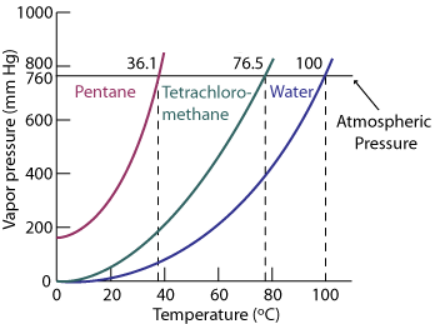
\includegraphics{vaporpressure}

\vspace{2em}
\subsection*{Question 2}
Below are qualitative descriptions of five solids. Classify each solid as amorphous, ionic crystalline, molecular crystalline, metallic crystalline, or covalent network solid

\begin{itemize}
  \item This solid has a high melting point and conducts electricity in both the liquid and solid phases

    \vspace{2em}
  \item This solid is an electrical insulator, and becomes soft and pliable over a temperature range rather than exhibiting a sharp melting point

    \vspace{2em}
  \item This solid is composed entirely of non-metal atoms. It has a very high melting point and is very hard. It does \emph{not} easily cleave along planes

    \vspace{2em}
  \item This solid is an insulator in both the solid and liquid phases. It has a moderate melting point

    \vspace{2em}
  \item This solid is an insulator, but conducts electricity when melted. It has a high melting point. The solid easily cleaves along planes

\end{itemize}

\newpage
\pagestyle{empty}
\addtocounter{page}{-1}
\section*{\emph{No Man Is an Island}}
\paragraph{John Donne}~
\begin{verse}
No man is an island, entire of itself;\\
every man is a piece of the continent,\\
a part of the main.\\

If a clod be washed away by the sea,\\
Europe is the less,\\
as well as if a promontory were,\\
as well as if a manor of thy friend’s\\
or of thine own were.\\

Any man’s death diminishes me,\\
because I am involved in mankind;\\
and therefore never send to know\\
for whom the bell tolls;\\
it tolls for thee.
\end{verse}
\end{document}
